\section{Powder sample components}
\label{powder}
In this section, we consider elastic coherent and incoherent
scattering from polycrystalline samples. We have chosen to
simulate the correct physical processes within the powder
samples on a quite detailed level.

\section{PowderN: A general powder sample}
\index{Samples!Powder, multiple diffraction line}
\index{Diffraction}

\component{Powder\_N}{System}{$r$, $h$, $\sigma_{\rm abs}$, $\sigma_{\rm inc}$, $V_0$, $f_{\rm pack}$, filename, DW}{}{validation in progress}

The powder diffraction component {\bf PowderN} models a powder sample
with background coming only from incoherent scattering and and no
multiple scattering. The description of the powder comes from a 
file in one of the standard output formats LAZY, FULLPROF, or CRYSTALLOGRAPHICA.

The sample has the shape of a solid cylinder, radius $r$ and height $h$.
The absorption and incoherent cross sections are given by 
$\sigma_c^a$ $\sigma_i,c^s$. 

The Bragg scattering from the powder,
$\sigma_c,c^a$ is calculated from the input file, with the parameters
$Q$, $|F(Q)|^2$, and $j$ for the scattering vector, structure factor, and
multiplicity, respectively. The volume of the unit cell is denoted $V_0$,
while the sample packing factor is $f_{\rm pack}$. 

%Further, the incoherent scattering is only taken into account
%by the attenuation of the beam, given by (\ref{e:attenu})
%and $\sigma_c^a$.
%The incoherently scattered neutrons are not
%propagated through to the detector, but rather not generated at all.

Focusing is performed by only scattering into one angular
interval, $d\phi$ of the Debye-Scherrer circle. The center of this
interval is located at the point where the Debye-Scherrer circle
intersects the half-plane defined by the initial velocity, ${\bf v}_{\rm i}$,
and a user-specified vector, {\bf f}.

%The input parameters for this component are
%
%\begin{quote}\begin{tabular}{ccl}
%$r$ & m & Radius of cylinder \\
%$h$ & m & Height of cylinder \\
%$\sigma_c^a$ & fm$^2$ & Absorption cross section per unit cell (at 2200 m/s) \\
%$\sigma_{i,c}^s$ & (fm)$^2$ & Incoherent scattering cross section per unit cell \\
%$\rho'/\rho$ & 1 & Packing factor \\
%$V_c$ & \AA$^3$ & Volume of unit cell \\
%${\bf Q}$ & \AA$^{-1}$ & The reciprocal lattice vector under consideration \\
%$|F({\bf Q}_j)|^2$ & (fm)$^2$ &
% Structure factor \\
%$j$ & 1 & Multiplicity of reflection \\
%$\exp(-2W)$ & 1 & Debye-Waller factor \\
%$d\phi$ & deg & Angular interval of focusing \\
%$f_x$ & m & \\
%$f_y$ & m & Focusing vector\\
%$f_z$ & m & \\
%\end{tabular}\end{quote}

\subsection{Powder scattering}
An ideal powder sample consists of many small
crystallites, although each crystallite is sufficiently
large not to cause measurable size broadening.
The orientation of the crystallites is evenly distributed,
and there is thus always a large number of
crystallites oriented to fulfill the Bragg condition
\begin{equation}   \label{Bragg}
n \lambda = 2 d \sin \theta ,
\end{equation}
where $n$ is the order of the scattering (an integer), $\lambda$
is the neutron wavelength, $d$ is the lattice spacing of the sample,
and $2 \theta$ is the scattering angle, see figure \ref{coneFig}.
As all crystal orientations
are realised in a powder sample, the neutrons are scattered within a
{\em Debye-Scherrer cone} of opening angle $4 \theta$ \cite{bacon}.

\begin{figure}
  \begin{center}
    \psfrag{2theta}[c][c]{$2\theta$}
    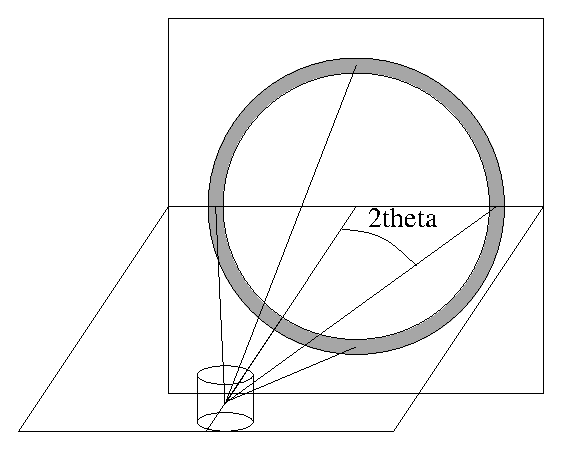
\includegraphics[width=0.6\textwidth]{figures/powder.eps}
  \end{center}
\caption{The scattering geometry of a powder sample showing part of the
Debye-Scherrer cone (solid lines) and the Debye-Scherrer circle (grey).}
\label{coneFig}
\end{figure}

Equation (\ref{Bragg}) may be cast into the form
\begin{equation}
|{\bf Q}| = 2 |{\bf k}| \sin \theta ,
\end{equation}
where {\bf Q} is a vector of the reciprocal lattice, and {\bf k} is
the wave vector of the neutron. It is seen that only
reciprocal vectors fulfilling $|{\bf Q}| < 2 |{\bf k}|$
contribute to the scattering.
For a complete treatment of the powder sample, one needs to take
into account all these {\bf Q}-values, since each of them contribute
to the attenuation.

The strength of the Bragg reflections is given by their structure factors
\begin{equation}
 \left| \sum_j b_j \exp({\bf R}_j \cdot {\bf Q}) \right|^2 ,
\end{equation}
where the sum runs over all atoms in one unit cell. This structure factor is
non-zero only when $Q$ equals a reciprocal lattice vector.

The textbook expression for the scattering cross section 
corresponding to one Debye-Scherrer cone reads \cite[ch.3.6]{squires}:
\begin{equation}
\sigma_{\rm cone} 
  = \frac{V}{V_0^2} \frac{\lambda^3}{4 \sin \theta} \sum_Q |F(Q)|^2 .
\end{equation}
For our purpose, this expression should be changed slightly. 
Firstly, the sum over structure factors for a particular $Q$ is replaced
by the sum over essentially different reflections multiplied by their
multiplicity, $j$. Then, a finite packing factor, $f$, is defined for the powder,
and finally, the Debye-Waller factor is multiplied on the elastic cross section
to take lattice vibrations into account (no inelastic background is simulated,
however). We then reach
\begin{equation}
\sigma_{\rm cone, Q} 
  = j_Q f \exp(-2W) \frac{V}{V_0^2} \frac{\lambda^3}{4 \sin \theta} |F(Q)|^2 ,
\end{equation}
in the thin sample approximation. For samples of finite thickness, the 
beam is being attenuated by the attenuation coefficient
\begin{equation}
\label{e:attenu}
\mu_{\rm Q} = \sigma_{\rm cone,Q} / V .
\end{equation}
For calibration it may be useful to consider the total intensity
scattered into a detector of effective height $h$, covering only
one reflection \cite[ch.3.6]{squires}.
A cut though the Debye-Scherrer cone perpendicular to its axis
is a circle. At the distance $r$ from the sample, the radius of this
circle is $r \sin(2\theta)$. Thus, the detector (in a small angle
approximation) counts a fraction $h / (2 \pi r \sin(2 \theta))$
of the scattered neutrons, giving a resulting count intensity:
\begin{equation}
I = \Psi \sigma_{\rm cone,Q} \frac{h}{2 \pi r \sin(2\theta)} , 
\end{equation}
where $\Psi$ is the flux at the sample position.

For clarity we repeat the meaning and unit of the symbols:
%
\begin{quote}\begin{tabular}{ccl}
$\Psi$ & s$^{-1}$m$^{-2}$ & Incoming intensity of neutrons \\
$I$    & s$^{-1}$ & Detected intensity of neutrons \\
$h$    & m        & Height of detector \\
$r$    & m        & Distance from sample to detector \\
$f$    & 1        & Packing factor of the powder \\
$j$    & 1        & Multiplicity of the reflection \\
$V_0$  & m$^{3}$  & Volume of unit cell\\
$|F({\bf Q})|^2$ & m$^2$  & Structure factor \\
$\exp(-2W)$ & 1  & Debye-Waller factor \\
$\mu_{\rm Q}$ & m$^{-1}$ & Linear attenuation factor due to scattering from
one powder line. \\
\end{tabular}\end{quote}
%
%Often, one defines the {\em scattering power} as
%\begin{equation}
%Q \equiv N^2 \frac{|F({\bf Q})|^2 \lambda^3}{V \sin(2\theta)}
% = N_c^2 V \frac{\rho'}{\rho} \frac{|F({\bf Q})|^2 \lambda^3}{\sin(2\theta)} ,
%\end{equation}
%where $N$ is the number of unit cells.

A powder sample will in general have several allowed reflections
${\bf Q}_j$, which will all contribute to the attenuation.
These reflections will have different values of
$|F({\bf Q}_j)|^2$ (and hence of $Q_j$), $j_j$, $\exp(-2W_j)$,
and $\theta_j$.
The total attenuation through the sample due to scattering is given by
$\mu^s = \mu_{\rm inc}^s + \sum_j \mu^s_j $,
where $\mu_{\rm inc}^s$ represents the incoherent scattering.

\subsection{Algorithm}
The algorithm of {\bf PowderN} can be summarized as
\begin{itemize}
\item Check if the neutron ray intersects the sample (otherwise ignore
the following).
\item Calculate the attenuation coefficients for scattering and absorption.
\item Perform Monte Carlo choices to determine the scattering position,
scattering type (coherent/incoherent), and the outgoing direction. 
\item Perform the necessary weight factor transformation.
\end{itemize}

\subsection{Calculating the weight factor}
